
\documentclass[a4paper,conference]{IEEEtran}
% Some Computer Society conferences also require the compsoc mode option,
% but others use the standard conference format.
%
% If IEEEtran.cls has not been installed into the LaTeX system files,
% manually specify the path to it like:
% \documentclass[conference]{../sty/IEEEtran}

\usepackage{cite}
\usepackage[pdftex]{graphicx}
\usepackage{amsmath}
\usepackage{algorithm2e}
\usepackage{subfigure}
\usepackage{threeparttable}
\usepackage{color}

\newcommand{\note}[1]{\textbf{\color{blue}#1}}

\begin{document}
%
% paper title
% Titles are generally capitalized except for words such as a, an, and, as,
% at, but, by, for, in, nor, of, on, or, the, to and up, which are usually
% not capitalized unless they are the first or last word of the title.
% Linebreaks \\ can be used within to get better formatting as desired.
% Do not put math or special symbols in the title.
\title{Image Sentiment Analysis\\ with Convolutional Networks}


% author names and affiliations
% use a multiple column layout for up to three different
% affiliations
\author{\IEEEauthorblockN{Zheng Lu, Yunhe Feng}
\IEEEauthorblockA{
Department of Electrical Engineering and Computer Science\\
University of Tennessee, Knoxville\\
Email: \{zlu12, yfeng14\}@vols.utk.edu}
}

% make the title area
\maketitle

% As a general rule, do not put math, special symbols or citations
% in the abstract
\begin{abstract}
Understanding the underlying attitude of people towards a given image automatically is important for many applications. The rapid growth of social media provides new opportunities and challenges to design image sentiment inference systems. Due to the weak relation between low-level visual features and sentiment, recent work focus on constructing mid-level semantic representation that can both be easily detected from the input images and be mapped to the sentiment class. However, ... We propose a novel convolution network based end to end system that can automatically generate the most suitable mid-level features. We show the effectiveness of our approaches by detecting sentiment of image tweets and show significant improvement against baseline approaches.
\end{abstract}

\IEEEpeerreviewmaketitle

\section{Introduction}
\label{introduction}

Recent years, social media platforms have seen a rapid growth of user-generated multimedia contents. Billion of images are shared on multiple social media platforms such as Instagram or Twitter which contributes to a large portion of the shared links. Through image sharing, users are usually also express their emotions and sentiments to strengthen the opinion carried in the content. Understanding users' sentiments provide us reliable signals of people's real-world activities which are very helpful in many applications such as predicting movie box-office revenues \cite{asur2010predicting}, political voting forecasts \cite{o2010tweets}. It can also be used as the building block for other tasks such as the image captioning \cite{vinyals2015show}.

Automatic sentiment analysis recognizes a person's position, attitude or opinion on an entity with computer technologies \cite{soleymani2017survey}. Text-based sentiment analysis has been the main concentration in the past. Only recently, sentiment analysis from online social media images has begun to draw more attentions. To simplify the task, previously, the sentiment analysis mainly focuses on the opinion's polarity, i.e., one's sentiment is classified into categories of positive, neutral and negative. 
However, as pointed out in many recent studies \cite{borth2013large, yuan2013sentribute, chen2014deepsentibank, ahsan2017towards}, it faces the unique challenge of large "affective gap" between the low-level features and the high-level sentiments. 

\begin{figure}[h]
    \centering
    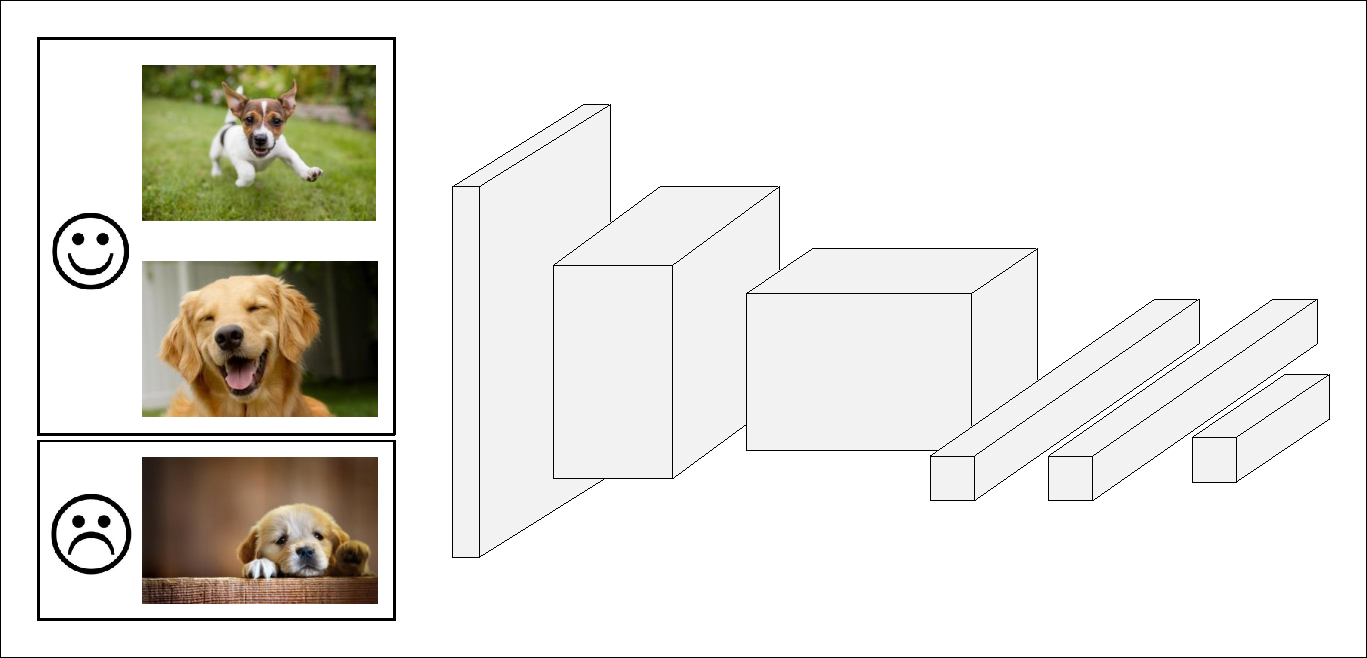
\includegraphics[width=\linewidth]{./figures/intro.pdf}
    \caption{Image sentiment analysis with triplet loss}
    \label{fig:intro}
\end{figure}

Recent work resort to extract manually designed mid-level representations from low-level features for image sentiment analysis tasks, e.g., visual sentiment ontology (VSO) in \cite{borth2013large}, mid-level attributes in \cite{yuan2013sentribute}. Such mid-level representations usually include both adjective and noun parts such as "happy dogs", "creepy house" and have strong sentiment. So approaches based on mid-level representations usually outperforms methods that inferring sentiment directly from low-level features. Rapid developments in Convolutional Neural Network (CNN) \cite{krizhevsky2012imagenet, szegedy2015going, simonyan2014very, he2016deep} push the transformations of computer vision tasks. There are also several efforts to apply CNN to image sentiment analysis \cite{you2015robust, chen2014deepsentibank, campos2017pixels}. However, recent works on applying convolutional networks still borrow the network architectures from the image classification tasks \cite{you2015robust, chen2014deepsentibank, ahsan2017towards, campos2017pixels}. Although convolutional neural networks are very effective at image classification tasks, they are not as effective when separating adjective parts that widely found in most mid-level representations for image sentiment analysis purpose.

To overcome this challenge, we first let the convolutional neural network trained on the noun part, then we adopt the triplet loss to replace surrogate loss used in the convolutional neural networks to force the network to focus more on the adjective part in the mid-level representations. When applying triplet loss, the network loot at three data points at the same time, the anchor point, the positive point and the negative point, where the anchor point and the positive point belongs to the same class and the negative point belongs to a different class. Then during training, the network tries to minimize the distance between anchor point and positive point and maximize the distance between the anchor point and the negative point.

A major challenge for triplet loss is mining triplets, as trivial triplets are not uninformative to the network and too hard triplets make the network hard to learn "normal" features \cite{hermans2017defense}. When applying triplet loss to mid-level representation classification for image sentiment analysis, we select triplets from the same noun class, with the anchor point and the positive point belongs to the same adjective class while negative point belongs to a different adjective class. In this way, the triplet loss forces the network to learn the adjective part of the mid-level representations and the triplets are informative and moderately hard for the network to learn.
  
\subsection{Contributions}
Our contributions can be summarized as follows:

\begin{itemize}
	\item We apply a two-stage learning scheme for the network to learn the adjective and noun part of mid-level representations in the image sentiment analysis separately;
	\item We replace surrogate loss in convolutional neural networks with triplet loss and design a triplet selection approach to force the network learn the adjective part of mid-level representations;
	\item We perform extensive experiments on several real word datasets to show the effectiveness of our approach in both mid-level representation classification and sentiment prediction.
\end{itemize}

The rest of this paper is organized as follows. In Section~\ref{relatedwork} we show previous works on image sentiment analysis.  
We explain our system structure and triplet selection scheme in Section~\ref{design}. 
The evaluations of our proposed method are in Section~\ref{evaluation}. 
We conclude our work in Section~\ref{conclusion}.

\section{Related Works}
\label{relatedwork} 

The majority of work in image sentiment analysis focus on manually design meaningful mid-level representations for the task for image sentiment prediction. \cite{borth2013large} trying to fill in the "affective gap" between the low-level features and the high-level sentiment by a set of mid-level representation called visual sentiment ontology that consists of more than 3,000 Adjective Noun Pairs (ANP) such as "beautiful flower" or "disgusting food". The authors also published a large-scale dataset called SentiBank that is widely used in later works. They also extend their work into a multilingual settings in one of their later work \cite{jou2015visual}. \cite{yuan2013sentribute} adopts a similar methodology as \cite{borth2013large}. The authors also construct a mid-level representations for better classification except that they choose different scene-based mid-level attributes than \cite{borth2013large}. In addition to that, they also include face detection to enhance the performance of images containing human faces. \cite{ahsan2017towards} studies the sentiment analysis of images of social events. It designs specific mid-level representations of each event class and classifies sentiment of each image without the help of texts associated with the image. Due to the challenge to manually collecting labeled data for image sentiment analysis, \cite{wang2015unsupervised} proposes an unsupervised method to facilitate social media images sentiment analysis with textual information associated with each image.

As convolutional neural networks are found to be very effective at image classification tasks, there are many efforts try to apply CNN to the image sentiment analysis task. \cite{chen2014deepsentibank} try to apply CNN based on AlexNet \cite{krizhevsky2012imagenet} to automatically extract features based on ANPs proposed in \cite{borth2013large}. \cite{you2015robust} also applies CNN to image sentiment analysis. They propose a method to progressively training CNN by keep training instances with distinct sentiment scores towards sentiment polars and discard training instances otherwise. \cite{campos2017pixels} studies how to fine-tune AlexNet-styled CNN to achieve better performance on image sentiment analysis tasks. 

Our work falls into the category of using convolutional networks to solve the image sentiment analysis task. Unlike previous works that mostly focus on modifying the neural network structure to increase the prediction accuracy, we adopt a different loss function, i.e., triplet loss \cite{hermans2017defense}, and modifying the training procedure to better detect mid-level representations in the input image.


\section{The design}
\label{design}

We propose to solve the ... .

\subsection{Preliminary}
In our problem ...

\subsection{Main design}

\subsection{More details}


\section{Evaluations}
\label{evaluation}

In this section, we show the results of experimental evaluation of ...

\subsection{Datasets}
\label{eval_datasets}

%\begin{table*}
		%\vspace{-0.5cm}
		%\caption{Datasets}
		%%\vspace{2 mm}
		%\label{table:datasets}
		%\begin{threeparttable}
			%\centering
			%\begin{tabular}{l|ccccccc} \hline
				%Dataset & size & mid-level size & class & workers & positive & neutral & negative \\ \hline
				%SentiBank-Flickr \cite{borth2013large} & ~316,000 & 1553 & N/A & auto & N/A & N/A & N/A \\ 
				%SentiBank-twitter \cite{borth2013large} & 603 & N/A & 2 & 3/3 & 470 & N/A & 133\\
				%twitter \cite{you2015robust} & 1269 & N/A & 2 & 3/5 & 769 & N/A & 500 \\
				%Bing \cite{ahsan2017towards} & 8,812 & 24 & 3 & 2/3 & 38.1\% & 48.1\% & 13.8\% \\ \hline
			%\end{tabular}
			%\begin{tablenotes}
				%\item Datasets with the no. of images and no. of mid-level representations if applicable. We also list how the label is generated, the number following manual method shows how many workers label each image. There are much more positive images than negative images as people tend to engage more with positive posts \cite{kramer2014experimental}.
			%\end{tablenotes}
		%\end{threeparttable}
		%\vspace{-0.3cm}
%\end{table*}

\begin{table}
		\vspace{-0.5cm}
		\caption{Datasets}
		\label{table:datasets}
		\begin{threeparttable}
			\centering
			\begin{tabular}{l|cccc} \hline
				Dataset & size & class & p/n & workers \\ \hline
				SentiBank-Flickr \cite{borth2013large} & ~316,000 & 1553 ANPs & N/A & auto \\ 
				SentiBank-twitter \cite{borth2013large} & 603 & 2 & 3.53 & 3/3 \\
				twitter \cite{you2015robust} & 1269 & 2 & 1.54 & 3/5\\
				Bing \cite{ahsan2017towards} & 8,812 & 3 & 2.76 & 2/3 \\ \hline
			\end{tabular}
			\begin{tablenotes}
				\item Datasets with the no. of images and no. of mid-level representations if applicable. We also list how the label is generated, the number following manual method shows how many workers label each image. There are much more positive images than negative images as people tend to engage more with positive posts \cite{kramer2014experimental}. We discard all the neutral images in all datasets.
			\end{tablenotes}
		\end{threeparttable}
		\vspace{-0.3cm}
\end{table}

We collect several public available data and list them in table \ref{table:datasets}. 

We evaluate our algorithm on ...

\subsection{Experiment settings}
\label{eval_system}

We evaluate our algorithms in ... setting

\subsection{Classification Accuracy}
\label{eval_accuracy}

We show the results...

\subsection{More}
\label{eval_more}


We show in this section that ...

\section{Conclusion}
\label{conclusion}

In this paper, we adopt a variant of convolutional neural networks with triplet loss to perform end-to-end learning that can automatically generate the most suitable mid-level features for image sentiment analysis tasks. We also designed a specific triplet selection schemes for mid-level representations commonly used in image sentiment analysis. We show the effectiveness of our approaches by detecting both mid-level representations and predicting sentiment of various image datasets and show significant improvement against baseline approaches.


% use section* for acknowledgment
%\section*{Acknowledgment}


%The authors would like to thank...

\bibliographystyle{abbrv}
\bibliography{reference}


% that's all folks
\end{document}


